\documentclass[12pt,a4paper]{article}

\usepackage[utf8]{inputenc}
\usepackage[T1]{fontenc}
\usepackage[english]{babel}
\usepackage{lmodern}
\usepackage{geometry}
\usepackage{microtype}
\usepackage{graphicx}
\usepackage{xcolor}
\usepackage{booktabs}
\usepackage{tabularx}
\usepackage{longtable}
\usepackage{array}
\usepackage{enumitem}
\usepackage{fancyhdr}
\usepackage{tikz}
\usepackage{hyperref}

\usetikzlibrary{arrows.meta,positioning,shapes.geometric}

\geometry{
    top=2.5cm,
    bottom=2.5cm,
    left=2.7cm,
    right=2.7cm
}

\definecolor{pinqevapink}{HTML}{D94F86}
\definecolor{pinqevadark}{HTML}{253044}
\definecolor{pinqevalight}{HTML}{F8EAF0}
\definecolor{implemented}{HTML}{2E7D32}
\definecolor{proposed}{HTML}{B26A00}

\hypersetup{
    colorlinks=true,
    linkcolor=pinqevadark,
    urlcolor=pinqevapink,
    citecolor=pinqevadark,
    pdftitle={Pinqeva System Architecture and Communication Protocol},
    pdfauthor={Pinqeva Project}
}

\pagestyle{fancy}
\fancyhf{}
\lhead{Pinqeva}
\rhead{System Architecture and Communication Protocol}
\cfoot{\thepage}
\setlength{\headheight}{15pt}
\setlength{\parindent}{0pt}
\setlength{\parskip}{0.7em}
\setlist[itemize]{topsep=0.3em,itemsep=0.25em}
\setlist[enumerate]{topsep=0.3em,itemsep=0.25em}
\renewcommand{\contentsname}{Índice}
\renewcommand{\arraystretch}{1.2}
\emergencystretch=2em

\newcommand{\currentstatus}{\textcolor{implemented}{\textbf{Current}}}
\newcommand{\proposedstatus}{\textcolor{proposed}{\textbf{Proposed}}}
\newcommand{\code}[1]{\texttt{#1}}

\begin{document}

\begin{titlepage}
    \centering
    \vspace*{2cm}

    {\Huge\bfseries\color{pinqevadark} Pinqeva\par}
    \vspace{0.4cm}
    {\Large Always know what is near.\par}

    \vspace{2cm}
    {\LARGE\bfseries System Architecture and\\[0.25cm]Communication Protocol\par}

    \vspace{1.5cm}
    \rule{0.8\textwidth}{0.5pt}

    \vspace{1.2cm}
    \begin{tabular}{rl}
        \textbf{Document version:} & 0.1 --- Draft \\
        \textbf{Date:} & 23 August 2026 \\
        \textbf{Project repository:} &
        \href{https://github.com/Th0masclassic/PROJECT_PINKEVA_TAG_w_SUBS}
        {PROJECT\_PINKEVA\_TAG\_w\_SUBS} \\
        \textbf{Purpose:} & Architecture baseline before client/server development
    \end{tabular}

    \vfill

    \begin{minipage}{0.86\textwidth}
        \centering
        \textit{This is a living architecture document. It explicitly separates
        behavior already implemented in the test project from behavior proposed
        for the complete Pinqeva product.}
    \end{minipage}

    \vspace{1cm}
\end{titlepage}

\section*{Motivation}
\addcontentsline{toc}{section}{Motivation}

People regularly misplace personal items such as wallets, keys, bags, cards,
and even parked vehicles. A compact Bluetooth tracker can help an owner identify
a nearby item and, when integrated with a compatible finder network, obtain
time-stamped location reports generated by participating devices.

A particularly useful Pinqeva scenario is leaving a tracker inside a car. The
application can remember the vehicle's information and show the latest reported
position on the Pinqeva map. This helps the owner find a parked car and may also
assist after theft. In that situation, compatible phones travelling inside or
passing near the stolen vehicle may anonymously relay the tracker's signal to
the finder network. Ironically, a compatible device carried by someone moving
with the vehicle may contribute to reporting the vehicle's location.

This is a crowd-sourced location mechanism rather than a covert, continuous GPS
system. Reports depend on nearby compatible devices, network availability, and
the finder service. They can be delayed or absent, and platform anti-stalking
protections may notify a person travelling with an unknown tracker. Pinqeva
must therefore display the report timestamp and must not promise an exact,
real-time, or guaranteed stolen-vehicle recovery service.

Pinqeva is motivated by the goal of combining this tracking capability with a
dedicated mobile experience, clear device ownership, an in-application map, and
subscription-controlled tracker operation and cloud services. An active
subscription is required for the tag to transmit its finder-network advertising
payload. The project is therefore not only
an embedded tracker. It is an end-to-end system composed of physical hardware,
firmware, a mobile client, a backend service, a database, subscription
management, an administration interface, and a map where an authenticated
owner can view the latest available position and location history.

Defining the architecture and protocol before implementing the client and
server reduces ambiguity between components. The firmware and mobile
application must agree on Bluetooth services, key sizes, message formats,
state transitions, result codes, and recovery behavior. The mobile application
and backend must also agree on authentication, device ownership, subscription
state, and location-report APIs.

The current repository contains ESP32 test firmware, experimental Apple Find My
report-retrieval scripts, an anisette test server, and a Supabase/PostgreSQL
schema for users, devices, ownership, plans, subscriptions, invoices, and
payment events. This document organizes these elements into one coherent target
architecture.

\clearpage
\tableofcontents
\clearpage

\section{Introduction}

\subsection{Purpose}

This document defines the hardware architecture, software architecture, and
communication boundaries of the Pinqeva tracker system. It is intended to guide
the next development stages: completing firmware provisioning, building the
mobile client, implementing the backend, and connecting the map and
subscription experience.

\subsection{Scope}

The complete system contains the following logical components:

\begin{itemize}
    \item A battery-powered Bluetooth tracker controlled by an ESP32-family
    microcontroller.
    \item Embedded firmware with setup and tracker operating modes.
    \item An iOS/Android client application for provisioning, management, and
    location display.
    \item A backend API responsible for authentication, device ownership, key
    lifecycle, subscriptions, and location access.
    \item A PostgreSQL database currently managed through Supabase.
    \item A background report worker that retrieves and processes
    finder-network location reports.
    \item A customer map interface for current and historical locations.
    \item An optional vehicle profile associated with a tracker, containing
    owner-provided details such as vehicle nickname, make, model, year, colour,
    and registration number.
    \item An administration interface for support and operational management.
    \item A payment-provider integration for subscription and invoice events.
\end{itemize}

Pinqeva must be described as a Bluetooth item tracker rather than an AirTag.
Apple Find My support is experimental in the current test project. A commercial
product requires the appropriate Apple program enrollment, approval,
anti-stalking behavior, and certification.

The tracker does not contain GNSS, cellular connectivity, or UWB. It therefore
does not independently calculate or transmit its global position. Nearby BLE
can provide discovery and a rough signal-strength indication. Global map
coordinates are obtained from compatible finder-network reports and processed
by the backend.

When the tracker is placed in a car, Pinqeva retrieves the latest location
report associated with the tag and combines it with the vehicle profile stored
in the application. The tag cannot retrieve vehicle telemetry such as speed,
fuel level, engine state, mileage, or diagnostic codes unless separate vehicle
hardware is added in the future.

\subsection{Document status terminology}

\begin{itemize}
    \item \currentstatus{} means the behavior exists in the checked-in test
    firmware or database migrations.
    \item \proposedstatus{} means the behavior is part of the target design but
    is not yet fully implemented.
\end{itemize}

\subsection{Architectural principles}

\begin{itemize}
    \item \textbf{BLE first:} the tracker communicates locally with the mobile
    application through Bluetooth Low Energy.
    \item \textbf{Least privilege:} users access only devices they actively own,
    while administrative functions require separate authorization.
    \item \textbf{Private-key isolation:} the private key used to decrypt
    location reports never enters the tracker and remains in protected
    server-side storage.
    \item \textbf{Explicit device states:} the firmware distinguishes
    unprovisioned, provisioning, active, subscription-suspended, error, and
    reset behavior.
    \item \textbf{Reliable provisioning:} the tracker becomes active only after
    validating, storing, and reading back its advertisement key.
    \item \textbf{Versioned contracts:} BLE and HTTPS protocols are versioned so
    the firmware, client, and backend can evolve safely.
    \item \textbf{Subscription enforcement:} an active, cryptographically signed
    entitlement is required before the firmware transmits the finder-network
    advertising payload.
    \item \textbf{Recoverable suspension:} an expired tag stops finder
    advertising but retains a minimal maintenance channel so the owner can
    renew and reactivate it.
\end{itemize}

\section{Hardware Architecture}

\subsection{Physical tracker}

The physical tracker is a compact battery-powered device intended to fit inside
or attach to personal belongings. At prototype level, its hardware consists of:

\begin{itemize}
    \item An ESP32-family microcontroller with Bluetooth Low Energy.
    \item Integrated flash storage for firmware and persistent provisioning
    data.
    \item A status LED connected to a GPIO output.
    \item A 2.4\,GHz antenna, integrated into the module or implemented on the
    PCB.
    \item A battery and power-regulation circuit.
    \item A programming and debugging connection used during development.
    \item Optional future hardware such as a buzzer, push button, battery
    monitor, or charging circuit.
\end{itemize}

The current test configuration targets the original Xtensa-based ESP32 with
2\,MB of flash. The wider product description refers to an ESP32-C3 reference
target. The final microcontroller must therefore be selected before the
production PCB is frozen. The BLE stack, GPIO mapping, memory usage, firmware
build, and power profile must be validated on that exact target.

\subsection{Hardware block diagram}

\begin{figure}[ht]
    \centering
    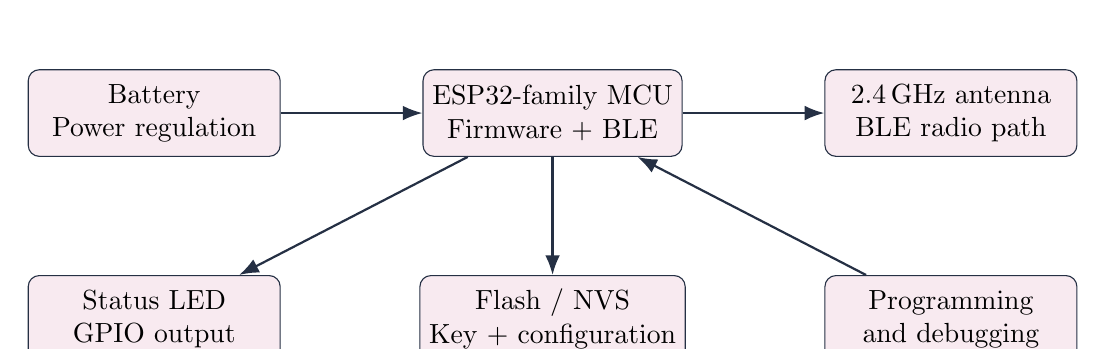
\begin{tikzpicture}[
        node distance=1.5cm and 1.8cm,
        block/.style={
            draw=pinqevadark,
            rounded corners,
            minimum width=3.2cm,
            minimum height=1.1cm,
            align=center,
            fill=pinqevalight
        },
        line/.style={-{Latex[length=2.5mm]},thick,pinqevadark}
    ]
        \node[block] (mcu) {ESP32-family MCU\\Firmware + BLE};
        \node[block, left=of mcu] (power) {Battery\\Power regulation};
        \node[block, right=of mcu] (antenna) {2.4\,GHz antenna\\BLE radio path};
        \node[block, below left=of mcu] (led) {Status LED\\GPIO output};
        \node[block, below=of mcu] (flash) {Flash / NVS\\Key + configuration};
        \node[block, below right=of mcu] (debug) {Programming\\and debugging};

        \draw[line] (power) -- (mcu);
        \draw[line] (mcu) -- (antenna);
        \draw[line] (mcu) -- (led);
        \draw[line] (mcu) -- (flash);
        \draw[line] (debug) -- (mcu);
    \end{tikzpicture}
    \caption{Prototype tracker hardware blocks.}
    \label{fig:hardware-blocks}
\end{figure}

\subsection{Microcontroller responsibilities}

The microcontroller is responsible for:

\begin{itemize}
    \item Initializing non-volatile storage and Bluetooth.
    \item Deriving a stable device identifier from the factory MAC address.
    \item Determining whether a valid 28-byte advertisement public key exists.
    \item Validating a signed subscription entitlement and its expiry time.
    \item Starting connectable setup advertising when the key is absent.
    \item Exposing the provisioning GATT service to the mobile application.
    \item Validating and persistently storing the advertisement key.
    \item Starting non-connectable tracker advertising only when provisioning
    is complete and the subscription entitlement is active.
    \item Stopping the finder-network payload when the entitlement expires.
    \item Controlling the status LED and reporting initialization errors.
\end{itemize}

The microcontroller does not process payments or decide whether a subscription
is paid. The backend remains authoritative for billing, while the
microcontroller enforces the signed entitlement issued by that backend. It is
also not responsible for user authentication, private-key storage, map
rendering, or global report retrieval.

\subsection{Bluetooth operating modes}

\begin{table}[ht]
    \centering
    \small
    \begin{tabularx}{\textwidth}{
        >{\bfseries}p{1.7cm}
        p{3.0cm}
        p{2.5cm}
        p{2.0cm}
        p{2.0cm}
        X
    }
        \toprule
        Mode & Advertising & Address & Interval & Connectable & Purpose \\
        \midrule
        Setup &
        BLE setup advertisement &
        Public address &
        100--250\,ms &
        Yes &
        Allow the mobile client to discover and provision a new tracker. \\

        Tracker &
        Finder-network advertisement &
        Random address derived from the public key &
        1--2\,s in the prototype &
        No &
        Broadcast the tracker payload while the signed subscription entitlement
        is active. \\

        Suspended &
        Maintenance/renewal advertisement only; no finder payload &
        Public or dedicated maintenance address &
        Low-duty-cycle &
        Yes &
        Allow subscription renewal without transmitting tracker advertising
        data. \\
        \bottomrule
    \end{tabularx}
    \caption{Bluetooth modes in the current prototype architecture.}
\end{table}

During setup, the current firmware advertises the name
\code{PKV-XXXXXXXXXXXX}, where the final twelve hexadecimal characters are
derived from the factory MAC address. This identifier supports discovery and
technical support, but it is not proof of ownership.

\subsection{Persistent storage}

\currentstatus{} The firmware initializes NVS and attempts to read the
advertisement key from a custom flash partition labelled \code{key}. Runtime
key writing and erased-value validation are not yet implemented.

\proposedstatus{} The storage module shall provide:

\begin{itemize}
    \item Atomic storage of the 28-byte advertisement key.
    \item A provisioning marker and storage-format version.
    \item Detection of erased values such as all \code{0xFF} bytes and invalid
    values such as all zeroes.
    \item Read-back verification before tracker activation.
    \item Controlled erase during an authorized factory reset.
    \item Compatibility with flash encryption in production.
\end{itemize}

NVS blob storage is suitable for the initial runtime implementation. A
dedicated encrypted partition can be adopted later if manufacturing or security
requirements justify it.

\subsection{LED feedback}

The status LED provides immediate feedback when no screen is available.
Production patterns remain configurable, but the architecture reserves these
meanings:

\begin{table}[ht]
    \centering
    \begin{tabularx}{0.9\textwidth}{p{4.5cm}X}
        \toprule
        \textbf{LED behavior} & \textbf{Meaning} \\
        \midrule
        Slow setup indication &
        Device is unprovisioned and waiting for the mobile application. \\
        Short confirmation pattern &
        Provisioning completed successfully. \\
        Repeated error pattern &
        Initialization, storage, or Bluetooth failure. \\
        Off during normal tracking &
        Tracker is operating normally and conserving power. \\
        \bottomrule
    \end{tabularx}
\end{table}

LED activity should be controlled by a task or timer so long visual patterns do
not block Bluetooth event processing.

\subsection{Power considerations}

BLE advertising interval, transmission power, LED duration, CPU wake time, and
the power-regulation circuit directly affect battery life. Persistent Wi-Fi or
MQTT connectivity is not part of the low-power tracker path. Battery-life
claims require measurements on the final PCB, antenna, battery, firmware, and
enclosure.

\section{Software Architecture}

\subsection{System overview}

\begin{figure}[ht]
    \centering
    \resizebox{\textwidth}{!}{
    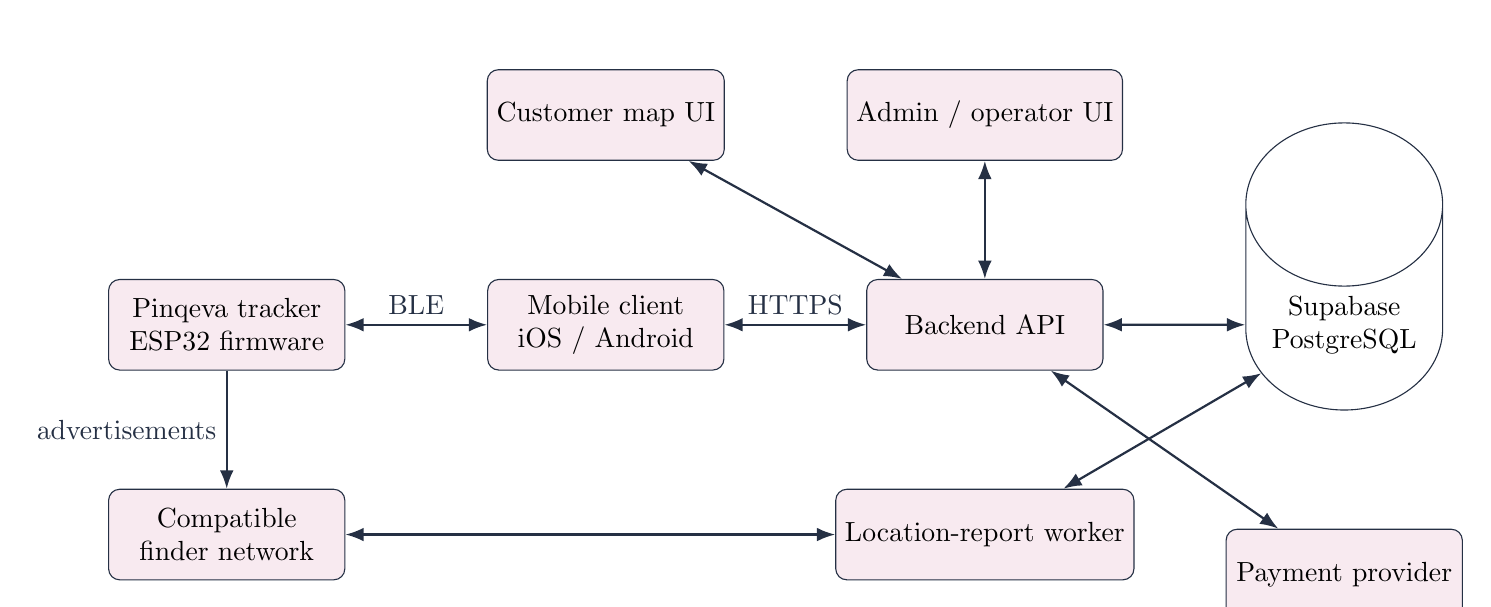
\begin{tikzpicture}[
        node distance=1.5cm and 1.8cm,
        component/.style={
            draw=pinqevadark,
            rounded corners,
            minimum width=3.0cm,
            minimum height=1.15cm,
            align=center,
            fill=pinqevalight
        },
        store/.style={
            cylinder,
            shape border rotate=90,
            draw=pinqevadark,
            minimum width=2.5cm,
            minimum height=1.4cm,
            align=center,
            fill=white
        },
        link/.style={<->,>=Latex,thick,pinqevadark},
        one/.style={->,>=Latex,thick,pinqevadark}
    ]
        \node[component] (tag) {Pinqeva tracker\\ESP32 firmware};
        \node[component, right=of tag] (mobile) {Mobile client\\iOS / Android};
        \node[component, right=of mobile] (api) {Backend API};
        \node[store, right=of api] (db) {Supabase\\PostgreSQL};

        \node[component, above=of api] (admin) {Admin / operator UI};
        \node[component, above=of mobile] (map) {Customer map UI};
        \node[component, below=of api] (worker) {Location-report worker};
        \node[component, below=of tag] (finder) {Compatible\\finder network};
        \node[component, below=of db] (payment) {Payment provider};

        \draw[link] (tag) -- node[above]{BLE} (mobile);
        \draw[link] (mobile) -- node[above]{HTTPS} (api);
        \draw[link] (api) -- (db);
        \draw[link] (admin) -- (api);
        \draw[link] (map) -- (api);
        \draw[link] (worker) -- (db);
        \draw[link] (worker) -- (finder);
        \draw[link] (api) -- (payment);
        \draw[one] (tag) -- node[left]{advertisements} (finder);
    \end{tikzpicture}
    }
    \caption{End-to-end Pinqeva software architecture.}
    \label{fig:system-architecture}
\end{figure}

The tracker communicates directly only with nearby BLE clients and the finder
network through its advertisements. It does not communicate directly with the
database, payment provider, administration interface, or map.

\subsection{Firmware architecture}

The firmware is divided into the following responsibilities:

\begin{itemize}
    \item \textbf{Application entry point:} initializes the LED and starts
    Bluetooth initialization in a FreeRTOS task.
    \item \textbf{BLE driver:} configures GAP advertising, registers GATT
    callbacks, manages connections, and selects setup or tracker behavior.
    \item \textbf{Storage driver:} initializes NVS and will provide validated
    key save, load, and erase operations.
    \item \textbf{Utility and LED module:} controls GPIO output and provides
    visible error feedback.
    \item \textbf{Provisioning service:} a proposed module that owns the GATT
    database, characteristic handles, protocol validation, and transition to
    tracker mode.
    \item \textbf{Entitlement verifier:} validates signed subscription leases,
    tracks their expiry, and suspends finder advertising when authorization is
    no longer valid.
\end{itemize}

\subsection{Firmware state model}

\begin{figure}[ht]
    \centering
    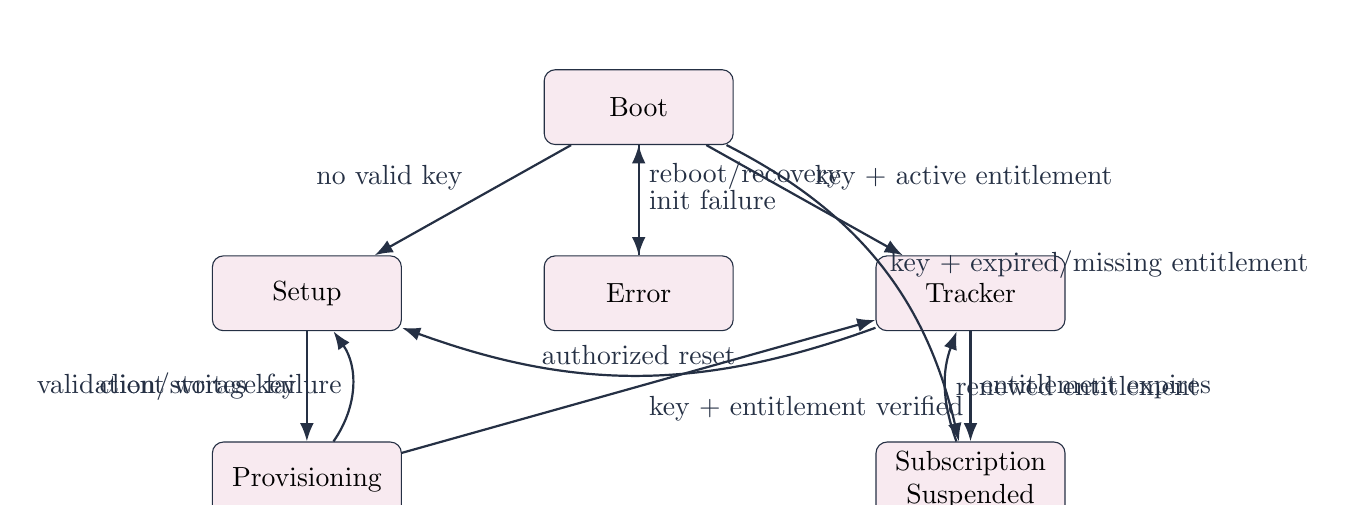
\begin{tikzpicture}[
        node distance=1.4cm and 1.8cm,
        state/.style={
            draw=pinqevadark,
            rounded corners,
            minimum width=2.4cm,
            minimum height=0.95cm,
            align=center,
            fill=pinqevalight
        },
        transition/.style={->,>=Latex,thick,pinqevadark}
    ]
        \node[state] (boot) {Boot};
        \node[state, below left=of boot] (setup) {Setup};
        \node[state, below=of boot] (error) {Error};
        \node[state, below right=of boot] (tracker) {Tracker};
        \node[state, below=of setup] (provisioning) {Provisioning};
        \node[state, below=of tracker] (suspended) {Subscription\\Suspended};

        \draw[transition] (boot) -- node[above left]{no valid key} (setup);
        \draw[transition] (boot) -- node[above right]{key + active entitlement} (tracker);
        \draw[transition] (boot) to[bend left=25]
            node[right]{key + expired/missing entitlement} (suspended);
        \draw[transition] (boot) -- node[right]{init failure} (error);
        \draw[transition] (setup) -- node[left]{client writes key} (provisioning);
        \draw[transition] (provisioning) -- node[below right]{key + entitlement verified} (tracker);
        \draw[transition] (provisioning) to[bend right=35]
            node[left]{validation/storage failure} (setup);
        \draw[transition] (tracker) -- node[right]{entitlement expires} (suspended);
        \draw[transition] (suspended) to[bend left=20]
            node[right]{renewed entitlement} (tracker);
        \draw[transition] (tracker) to[bend left=20]
            node[above]{authorized reset} (setup);
        \draw[transition] (error) -- node[above right]{reboot/recovery} (boot);
    \end{tikzpicture}
    \caption{Firmware state transitions.}
\end{figure}

\subsection{Mobile client application}

The mobile client acts as the BLE central and GATT client. It is responsible
for:

\begin{itemize}
    \item User registration, login, and session management.
    \item Scanning for setup-mode devices advertising the Pinqeva service.
    \item Connecting to the selected tracker.
    \item Reading the device identifier, firmware version, and protocol version.
    \item Requesting a provisioning public key from the backend.
    \item Requesting the signed subscription entitlement for the selected
    device.
    \item Writing only the 28-byte advertisement public key to the tracker.
    \item Writing or refreshing the signed entitlement through BLE.
    \item Waiting for explicit success before displaying completion.
    \item Registering the device and ownership relationship with the backend.
    \item Displaying owned devices, subscription status, latest location, and
    location history.
    \item Rendering the location inside the Pinqeva map UI.
    \item Allowing the owner to classify a tracker as a vehicle tracker and
    store or retrieve the associated vehicle profile.
    \item Displaying vehicle location freshness, including the observation time
    and whether the car is currently nearby or only has a historical report.
    \item Supporting future nearby actions such as ringing the tracker.
\end{itemize}

The application must not infer global location from BLE signal strength.
Received Signal Strength Indicator (RSSI) can support a rough nearby indication,
whereas global map coordinates come from the backend.

\subsection{Backend API}

The backend is the authority for identity, ownership, subscriptions, and
location access. It is responsible for:

\begin{itemize}
    \item Authenticating users and validating sessions.
    \item Creating short-lived provisioning sessions.
    \item Generating or securely importing finder-network key pairs.
    \item Keeping private keys in protected server-side storage.
    \item Returning only the advertisement public key to the authorized client.
    \item Issuing a device-bound, signed entitlement whose expiry matches the
    paid subscription period.
    \item Binding a device identifier to its owner after successful
    provisioning.
    \item Enforcing ownership checks on every device and location request.
    \item Exposing device, map, plan, subscription, invoice, and account APIs.
    \item Receiving signed and idempotent payment webhooks.
    \item Writing auditable administrative and security events.
    \item Coordinating the location-report worker.
\end{itemize}

The mobile application must never contain database administrator credentials,
payment-provider secrets, or server private keys.

\subsection{Location-report worker and map}

The location-report worker retrieves encrypted reports from the compatible
finder network, matches each report to a device key, decrypts the report
server-side, validates its timestamp and coordinate range, and stores a
normalized location record.

The map UI requests the latest location or a bounded history from the backend.
A response should contain latitude, longitude, observation time, confidence or
accuracy information when available, and an indication that the value is a
historical crowd-sourced report rather than a real-time GPS position.

For a tracker assigned to a car, the map presents the vehicle profile together
with the latest report. The main vehicle screen should show the vehicle name,
make/model, registration number when the owner chooses to store it, last
reported coordinates, observation time, report age, and a clear
\textit{last reported} status. Location history may show movement between
reports, but it must not draw an invented continuous route between sparse
observations.

In a possible theft scenario, the backend continues processing reports received
for the tracker. Compatible devices in or near the moving car may anonymously
relay its Bluetooth advertisement. This can help the owner provide recent
information to the appropriate authorities, but Pinqeva should advise users not
to confront a suspected thief or attempt recovery themselves.

The database requires a future location table containing, at minimum:

\begin{itemize}
    \item \code{id} and \code{device\_id};
    \item \code{observed\_at} and \code{received\_at};
    \item \code{latitude} and \code{longitude};
    \item confidence or accuracy metadata;
    \item report source;
    \item protected raw-report metadata only when retention is justified.
\end{itemize}

The database also requires an optional vehicle profile associated one-to-one
with a device. A proposed \code{vehicle\_profile} record contains:

\begin{itemize}
    \item \code{device\_id};
    \item owner-defined vehicle nickname;
    \item make, model, year, and colour;
    \item registration number, stored only when the owner chooses to provide it;
    \item optional notes useful for identifying the vehicle;
    \item creation and update timestamps.
\end{itemize}

Vehicle profile data follows the same ownership rules as the tracker. A user
cannot read or modify vehicle information associated with another user's
device. Registration numbers and precise location history are personal data and
require appropriate protection.

Location history is sensitive personal data. Retention, export, deletion,
encryption, and exceptional-access policies must be defined before production.

\subsection{Database architecture}

The existing Supabase migrations define the entities in
Table~\ref{tab:database-entities}.

\begin{table}[ht]
    \centering
    \begin{tabularx}{\textwidth}{>{\ttfamily}p{3.2cm}X}
        \toprule
        \normalfont\textbf{Entity} & \textbf{Responsibility} \\
        \midrule
        profiles &
        Application profile linked to a Supabase authenticated user. \\
        device &
        Tracker identity, name, status, and firmware version. \\
        ownership &
        Time-bounded relationship between a user and a device. \\
        plan &
        Available subscription plan, duration, and price. \\
        subscription &
        User/device entitlement and billing period. \\
        invoice &
        Financial record associated with a subscription. \\
        payment\_event &
        Idempotent record of payment-provider webhook events. \\
        \bottomrule
    \end{tabularx}
    \caption{Current application database entities.}
    \label{tab:database-entities}
\end{table}

Row Level Security currently limits profile, ownership, and device reads to the
authenticated user. Before production, policies must also protect
subscriptions, invoices, location reports, provisioning sessions, and future
tables. A device must have at most one active ownership record, and ownership
transfer must be explicit and audited.

\subsection{Subscription architecture}

Subscriptions are associated with both a user and a device. This allows one
customer to own several trackers with different plan periods. An active
subscription is required to use a Pinqeva tag as a finder-network tracker.

The backend is authoritative for billing and issues a cryptographically signed,
device-bound entitlement after confirming payment. The mobile application
transfers this entitlement to the tag through BLE. The firmware verifies the
signature using an embedded backend public key and transmits finder advertising
data only until the entitlement expiry.

When the entitlement expires, the firmware enters \textit{Subscription
Suspended} mode and stops transmitting the finder-network payload. The stored
advertisement key is retained. The tag exposes only a low-duty-cycle
maintenance/renewal advertisement that does not include the finder payload,
allowing the authenticated owner to reconnect after payment and install a new
entitlement.

The tag has no permanent Internet connection and therefore cannot query the
backend at the instant a subscription changes. Local enforcement uses the
signed expiry time. The entitlement can remain valid until the paid
\code{current\_period\_end}; cancellation at period end therefore does not stop
an already-paid period. Immediate revocation requires a later BLE
synchronization unless future hardware provides an independent secure network
and time source.

Secure expiry enforcement also requires trustworthy time. While continuously
powered, the firmware can combine the last authenticated UTC value with a
monotonic timer. After a power loss or clock rollback, the secure behavior is
fail-closed: the tag remains suspended until the authenticated application
installs a fresh entitlement and trusted time value.

Payment webhooks must be signature-verified and idempotent before changing
subscription state or issuing an entitlement. Reset, renewal, safety behavior,
anti-stalking behavior, and critical firmware recovery remain available in
suspended mode even though finder advertising is disabled.

\subsection{Administration and operator interface}

Administration belongs in the software architecture because operators interact
with users, devices, subscriptions, payments, and support cases. It does not
require a separate hardware protocol.

The administration interface should use a separate authorization domain with
role-based access control and multi-factor authentication. It may provide:

\begin{itemize}
    \item Device lookup by internal ID or serial number.
    \item Firmware and last-seen status.
    \item Ownership history without silent ownership reassignment.
    \item Subscription, invoice, and payment-event status.
    \item Audited support actions such as session revocation or reset approval.
    \item Security and operational audit events.
\end{itemize}

Administrators should not routinely view private keys or precise location
history. Exceptional access must have a defined support purpose and produce an
audit record.

\subsection{Security boundaries}

The most important trust boundaries are:

\begin{itemize}
    \item Between an unknown nearby phone and a setup-mode tracker.
    \item Between the mobile application and the backend API.
    \item Between ordinary users and administrative functions.
    \item Between application services and private-key storage.
    \item Between the payment provider and webhook receiver.
    \item Between location data and any requester.
\end{itemize}

A production tracker should require physical presence or a setup secret printed
as a QR code to prevent a nearby attacker from claiming a new device. BLE
encryption and bonding should protect provisioning. The initial prototype may
use a simplified test flow, but that behavior is not production security.

\section{Communication Protocol}

\subsection{Communication interfaces}

\begin{table}[ht]
    \centering
    \small
    \begin{tabularx}{\textwidth}{p{2.6cm}p{2.6cm}p{4.0cm}X}
        \toprule
        \textbf{Interface} & \textbf{Transport} &
        \textbf{Participants} & \textbf{Purpose} \\
        \midrule
        Provisioning &
        BLE GATT &
        Mobile client and tracker &
        Identify and activate a new tracker. \\
        Nearby control &
        BLE GATT &
        Mobile client and tracker &
        Future status, ring, reset, and diagnostics. \\
        Application API &
        HTTPS with JSON &
        Mobile, map, admin, and backend &
        Authentication, devices, subscriptions, and locations. \\
        Database &
        PostgreSQL protocol &
        Backend, worker, and database &
        Durable application state. \\
        Report retrieval &
        HTTPS &
        Worker and finder service &
        Retrieve encrypted location reports. \\
        Payments &
        HTTPS API/webhooks &
        Backend and payment provider &
        Subscription and invoice lifecycle. \\
        \bottomrule
    \end{tabularx}
\end{table}

\subsection{Setup advertising protocol}

An unprovisioned tracker sends a connectable BLE advertisement containing the
standard flags and complete local name \code{PKV-XXXXXXXXXXXX}. The target
implementation also advertises the Pinqeva Provisioning Service UUID so the
client does not rely only on a name prefix.

The client scans for the service UUID, displays candidate device identifiers,
and connects after user selection. Setup advertising resumes after an
unexpected disconnect while the device remains unprovisioned.

\subsection{Proposed Pinqeva Provisioning GATT service}

The UUIDs in Table~\ref{tab:gatt-service} define protocol version 1. They are
proposed values and should become stable when both firmware and client start
using them.

\begin{longtable}{p{3.2cm}p{5.0cm}p{3.1cm}p{3.2cm}}
    \caption{Proposed Pinqeva Provisioning Service.}
    \label{tab:gatt-service} \\
    \toprule
    \textbf{Attribute} & \textbf{UUID} & \textbf{Properties} &
    \textbf{Value} \\
    \midrule
    \endfirsthead

    \toprule
    \textbf{Attribute} & \textbf{UUID} & \textbf{Properties} &
    \textbf{Value} \\
    \midrule
    \endhead

    Provisioning Service &
    \code{a6f0f000-3e4d-4b1a-9c2e-72d24c8f0a01} &
    Primary service &
    Contains all provisioning characteristics. \\

    Protocol Information &
    \code{a6f0f001-3e4d-4b1a-9c2e-72d24c8f0a01} &
    Read &
    Protocol version, firmware version, and capabilities. \\

    Device Identifier &
    \code{a6f0f002-3e4d-4b1a-9c2e-72d24c8f0a01} &
    Read &
    UTF-8 \code{PKV-XXXXXXXXXXXX}. \\

    Advertisement Key &
    \code{a6f0f003-3e4d-4b1a-9c2e-72d24c8f0a01} &
    Write with response &
    Exactly 28 raw binary bytes. \\

    Provisioning Status &
    \code{a6f0f004-3e4d-4b1a-9c2e-72d24c8f0a01} &
    Read and Notify &
    Current state and result code. \\

    Device Command &
    \code{a6f0f005-3e4d-4b1a-9c2e-72d24c8f0a01} &
    Write with response &
    Versioned commands such as commit or authorized reset. \\

    Subscription Entitlement &
    \code{a6f0f006-3e4d-4b1a-9c2e-72d24c8f0a01} &
    Write with response, Read status &
    Signed device-bound entitlement and expiry. \\
    \bottomrule
\end{longtable}

The key is transferred as raw binary rather than Base64 text. The client checks
the platform's maximum write length. When a single 28-byte write is not
supported by the negotiated ATT MTU, the client and firmware use a prepared or
long write. Partial, uncommitted data must never replace a stored key.

\subsection{Protocol Information value}

Protocol Information uses the compact binary value below.

\begin{table}[ht]
    \centering
    \begin{tabular}{ccc}
        \toprule
        \textbf{Offset} & \textbf{Size} & \textbf{Field} \\
        \midrule
        0 & 1 byte & Protocol major version \\
        1 & 1 byte & Protocol minor version \\
        2 & 1 byte & Firmware major version \\
        3 & 1 byte & Firmware minor version \\
        4 & 2 bytes & Capability flags, little-endian \\
        \bottomrule
    \end{tabular}
\end{table}

An incompatible major version stops provisioning. A newer minor version can be
accepted when the required characteristics and capability flags are present.

\subsection{Provisioning Status value}

Provisioning Status contains two bytes: one state byte followed by one result
byte.

\begin{table}[ht]
    \centering
    \begin{tabularx}{0.9\textwidth}{p{3.2cm}p{2.0cm}X}
        \toprule
        \textbf{State} & \textbf{Value} & \textbf{Meaning} \\
        \midrule
        Unprovisioned & \code{0x00} & No valid stored key. \\
        Receiving & \code{0x01} & Key write is in progress. \\
        Validating & \code{0x02} & Completed value is being validated. \\
        Persisting & \code{0x03} & Key is being written and read back. \\
        Ready & \code{0x04} & Provisioning succeeded. \\
        Suspended & \code{0x05} & Finder advertising disabled because no active entitlement exists. \\
        Error & \code{0x7F} & Result byte identifies the failure. \\
        \bottomrule
    \end{tabularx}
\end{table}

\begin{table}[ht]
    \centering
    \begin{tabularx}{0.9\textwidth}{p{3.2cm}p{2.0cm}X}
        \toprule
        \textbf{Result} & \textbf{Value} & \textbf{Meaning} \\
        \midrule
        Success & \code{0x00} & Operation completed. \\
        Invalid length & \code{0x01} & Key is not exactly 28 bytes. \\
        Invalid value & \code{0x02} & Key value is erased or rejected. \\
        Storage failure & \code{0x03} & Save or read-back failed. \\
        Already provisioned & \code{0x04} & Replacement is not allowed. \\
        Unauthorized & \code{0x05} & Setup proof is insufficient. \\
        Unsupported version & \code{0x06} & Protocol versions are incompatible. \\
        Entitlement rejected & \code{0x07} & Entitlement is invalid, expired, or for another device. \\
        Internal error & \code{0x7F} & Unclassified firmware failure. \\
        \bottomrule
    \end{tabularx}
\end{table}

\subsection{Key lifecycle}

The finder key pair contains a private key and a 28-byte advertisement public
key. Their lifecycle is deliberately separated:

\begin{enumerate}
    \item The backend generates or securely imports the key pair for an
    authenticated provisioning session.
    \item The backend stores the private key in protected server-side storage.
    \item The backend sends only the advertisement public key to the
    authenticated mobile client.
    \item The mobile client transfers the public key to the selected tracker
    over the protected BLE connection.
    \item The tracker validates, stores, and reads back the public key.
    \item The tracker derives its random BLE address and advertising payload
    from that public key.
    \item The backend later uses the private key to decrypt reports associated
    with the public-key identifier.
\end{enumerate}

The private key must never be written to the tracker, displayed in the
administration interface, logged, or stored in ordinary mobile application
storage.

\subsection{Subscription entitlement protocol}

The subscription entitlement is a signed lease rather than a Boolean value sent
by the application. A version-1 entitlement contains:

\begin{itemize}
    \item entitlement format version;
    \item device identifier;
    \item subscription identifier;
    \item validity start and expiry timestamps in UTC;
    \item monotonically increasing issuance counter or unique nonce;
    \item permitted capability flags;
    \item backend signature over every preceding field.
\end{itemize}

The firmware contains only the backend's public verification key. It verifies
the signature, device binding, anti-rollback counter, and expiry before storing
the entitlement. The backend signing key never enters the mobile application or
tracker. A successfully verified renewal replaces the previous entitlement
atomically and allows tracker advertising to restart.

The active tag needs a defined maintenance mechanism so the app can install
renewals before expiry. The production design may use short periodic
connectable maintenance windows or a physical action that temporarily enables
the GATT service. Suspended mode always provides a low-duty-cycle renewal
window, but never includes the finder-network advertisement key.

\subsection{Provisioning sequence}

\begin{figure}[ht]
    \centering
    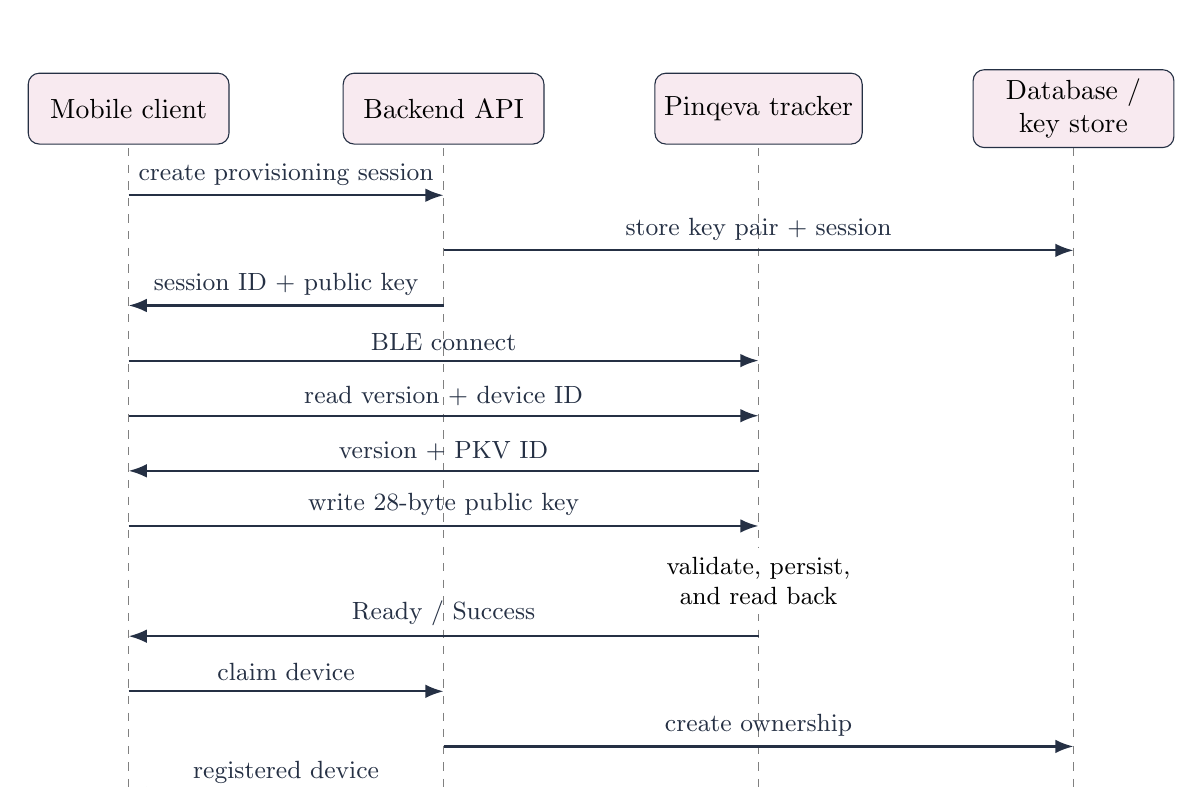
\begin{tikzpicture}[
        participant/.style={
            draw=pinqevadark,
            rounded corners,
            minimum width=2.55cm,
            minimum height=0.9cm,
            align=center,
            fill=pinqevalight
        },
        msg/.style={->,>=Latex,thick,pinqevadark},
        note/.style={font=\small,align=center}
    ]
        \node[participant] (app) at (0,0) {Mobile client};
        \node[participant] (api) at (4,0) {Backend API};
        \node[participant] (tag) at (8,0) {Pinqeva tracker};
        \node[participant] (db) at (12,0) {Database /\\key store};

        \foreach \x in {0,4,8,12}
            \draw[dashed,gray] (\x,-0.5) -- (\x,-8.7);

        \draw[msg] (0,-1.1) -- node[above,note]{create provisioning session} (4,-1.1);
        \draw[msg] (4,-1.8) -- node[above,note]{store key pair + session} (12,-1.8);
        \draw[msg] (4,-2.5) -- node[above,note]{session ID + public key} (0,-2.5);
        \draw[msg] (0,-3.2) -- node[above,note]{BLE connect} (8,-3.2);
        \draw[msg] (0,-3.9) -- node[above,note]{read version + device ID} (8,-3.9);
        \draw[msg] (8,-4.6) -- node[above,note]{version + PKV ID} (0,-4.6);
        \draw[msg] (0,-5.3) -- node[above,note]{write 28-byte public key} (8,-5.3);
        \node[note,fill=white] at (8,-6.0) {validate, persist,\\and read back};
        \draw[msg] (8,-6.7) -- node[above,note]{Ready / Success} (0,-6.7);
        \draw[msg] (0,-7.4) -- node[above,note]{claim device} (4,-7.4);
        \draw[msg] (4,-8.1) -- node[above,note]{create ownership} (12,-8.1);
        \draw[msg] (4,-8.7) -- node[above,note]{registered device} (0,-8.7);
    \end{tikzpicture}
    \caption{Proposed end-to-end provisioning sequence.}
\end{figure}

If the BLE operation succeeds but the API claim fails, the client retries the
same idempotent claim rather than generating a new key. Provisioning sessions
therefore require a unique identifier, expiry, single-device binding, and
idempotent completion.

\subsection{Tracker advertising protocol}

\currentstatus{} After provisioning, the firmware constructs a 31-byte
manufacturer-specific BLE advertisement using Apple company identifier
\code{0x004C}, offline-finding type \code{0x12}, and length \code{0x19}. It
derives the random BLE address from the first six public-key bytes and places
the remaining key material in the advertisement payload.

Tracker advertising is non-connectable in the prototype. Future nearby commands
would require a controlled connectable window, maintenance mode, or alternative
scheduling strategy. That choice affects both battery life and security.

\subsection{Application HTTPS API}

The exact implementation can evolve, but the logical version-1 operations are:

\begin{longtable}{p{4.0cm}p{5.3cm}p{5.0cm}}
    \caption{Proposed application API.} \\
    \toprule
    \textbf{Operation} & \textbf{Example route} & \textbf{Authorization} \\
    \midrule
    \endfirsthead
    \toprule
    \textbf{Operation} & \textbf{Example route} & \textbf{Authorization} \\
    \midrule
    \endhead

    Create provisioning session &
    \code{POST /v1/provisioning-sessions} &
    Authenticated user \\

    Complete device claim &
    \code{POST /v1/devices/claim} &
    Provisioning-session owner \\

    List owned devices &
    \code{GET /v1/devices} &
    Authenticated owner \\

    Read one device &
    \code{GET /v1/devices/\{deviceId\}} &
    Active owner or authorized operator \\

    Rename device &
    \code{PATCH /v1/devices/\{deviceId\}} &
    Active owner \\

    Read vehicle profile &
    \code{GET /v1/devices/\{deviceId\}/vehicle} &
    Active owner \\

    Create or update vehicle profile &
    \code{PUT /v1/devices/\{deviceId\}/vehicle} &
    Active owner \\

    Latest location &
    \code{GET /v1/devices/\{deviceId\}/locations/latest} &
    Active owner with applicable entitlement \\

    Location history &
    \code{GET /v1/devices/\{deviceId\}/locations} &
    Active owner with applicable entitlement \\

    List plans &
    \code{GET /v1/plans} &
    Public or authenticated according to policy \\

    Manage subscription &
    \code{POST /v1/subscriptions} &
    Authenticated owner \\

    Issue/refresh tag entitlement &
    \code{POST /v1/devices/\{deviceId\}/entitlements} &
    Active owner with a paid subscription \\

    Payment webhook &
    \code{POST /v1/webhooks/payments} &
    Valid payment-provider signature \\
    \bottomrule
\end{longtable}

All application traffic uses HTTPS and schema-validated JSON. Ownership is
checked server-side. Provisioning and payment retries use idempotency keys.
Precise coordinates are never returned for a device the requester does not
actively own.

\subsection{Failure and recovery behavior}

\begin{itemize}
    \item A device with no valid key remains in setup mode.
    \item An interrupted transfer leaves the previous valid key unchanged.
    \item An invalid key produces an explicit error and does not activate
    tracker mode.
    \item A storage failure keeps the device in setup mode and activates an
    error indication.
    \item An unexpected disconnect restarts setup advertising.
    \item A provisioned device rejects key replacement unless an authorized
    reset flow is active.
    \item A missing, invalid, or expired entitlement prevents finder-network
    advertising even when a valid public key is stored.
    \item Suspended mode retains the public key and exposes only the renewal
    channel.
    \item A renewed signed entitlement atomically reactivates tracker
    advertising after verification.
    \item A reboot without trustworthy time fails closed into suspended mode
    until the app provides a fresh signed entitlement and trusted time.
    \item Success is reported only after persistent read-back verification.
    \item Backend claim completion is idempotent so retries cannot create
    duplicate ownership records.
    \item Factory reset clears the public key and ownership binding through an
    explicit, auditable process.
\end{itemize}

\section{Current Implementation Status and Next Milestone}

\subsection{Implemented in the repository}

\begin{itemize}
    \item ESP32 application startup and FreeRTOS Bluetooth initialization task.
    \item GPIO LED initialization and blink/error utility.
    \item Device identifier derived from the factory MAC address.
    \item Setup and tracker firmware modes.
    \item Connectable setup advertisement with the \code{PKV-} device name.
    \item Non-connectable tracker advertisement built from a 28-byte public key.
    \item GAP and GATT callback registration with event logging.
    \item Basic NVS initialization and key reading from a custom partition.
    \item Experimental key generation and report-retrieval scripts.
    \item Supabase tables for profiles, devices, ownership, plans,
    subscriptions, invoices, and payment events.
    \item Initial Row Level Security for profiles, ownership, and devices.
\end{itemize}

\subsection{Not yet implemented or incomplete}

\begin{itemize}
    \item Creation of the Pinqeva GATT service and characteristics.
    \item Runtime key validation, storage, read-back, and erase operations.
    \item Actual handling of the advertisement-key write callback.
    \item Secure BLE pairing and production anti-claim protection.
    \item Mobile client application in the current checked-in tree.
    \item Backend provisioning and device-claim API in the current tree.
    \item Secure private-key storage and report-worker integration.
    \item Location-report schema and Pinqeva map implementation.
    \item Vehicle profile schema, API, and vehicle-focused map experience.
    \item Signed subscription-entitlement issuance, BLE synchronization,
    trusted-time handling, firmware enforcement, and payment-provider
    integration.
    \item Administrative roles, policies, audit events, and operator UI.
    \item Production power, RF, security, anti-stalking, and certification tests.
\end{itemize}

\subsection{Next milestone}

The next milestone is one complete provisioning vertical slice:

\begin{enumerate}
    \item Implement the proposed GATT service in the firmware.
    \item Implement atomic save, load, and erase operations for the public key
    and signed entitlement.
    \item Implement entitlement verification and the subscription-suspended
    state.
    \item Validate the flow manually with a BLE test client.
    \item Build the minimum mobile screen for scan, connect, read, write, and
    confirmation.
    \item Reboot the tracker and verify that it enters tracker mode only with
    both a stored key and an active entitlement.
    \item Verify that an expired entitlement stops the finder payload while the
    renewal channel remains available.
    \item Add an idempotent backend device-claim operation and create the
    ownership record.
\end{enumerate}

The milestone is complete when a blank tracker can be provisioned from the
mobile client, receives a signed entitlement, survives a reboot, broadcasts the
expected tracker payload only during the paid period, enters suspended mode
after expiry, can be renewed, and appears under the correct authenticated
account.

\section{Conclusion}

Pinqeva is an end-to-end Bluetooth tracking platform rather than only an
embedded firmware project. The same tag can protect personal items or be
assigned to a vehicle, allowing the application to combine owner-provided car
information with the latest crowd-sourced location report. In the event of
vehicle theft, compatible devices travelling with or passing near the car may
help report the tag's changing location, although availability and timing are
not guaranteed.

The architecture separates low-power hardware from mobile onboarding, cloud
location processing, subscriptions, vehicle and map presentation, and
administration. The tracker stores the advertisement public key and a signed
subscription entitlement, while the backend protects the private key and
controls entitlement issuance.

The current firmware already distinguishes a device with a stored public key
from one that must enter setup mode. The target state decision adds a mandatory
subscription check: only a valid key together with an active signed entitlement
permits finder advertising. The immediate engineering task is to complete the
provisioning and entitlement protocol that bridges these states. After that
contract is tested, the client and backend can be developed against a stable,
documented interface.

\end{document}
